\section{System Overview (75 pts)\label{sec:1}}

    \begin{figure}
        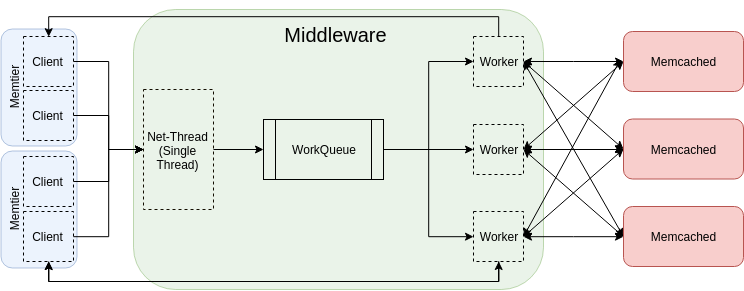
\includegraphics[width=0.8\linewidth]{graphics/system-request-flow.png}
        \caption{Basic flow of information in the system. Each box with a dashed border indicates a thread on the
                 respective system which are colour coded into 3 categories, blue for \cli, green for \mw{} and red for
                 \srv. Arrows denote the order of flow of information.\label{fig:request-overview}}
    \end{figure}

    The basic flow of requests through the system is visualized in figure \ref{fig:request-overview}. A basic lifetime
    of a request begins in a thread on a middleware, is received by the Net-Thread and upon receiving a complete packet
    it is stored in the WorkQueue. This queue is shared for any threads in the middleware and they compete for each
    individual element. The moment a Worker receives the request it processes it locally, infers the type and first
    sends the request to either one connected memcached (non-sharded GET) or all connected memcached instances connected
    (sharded GET and SET). Upon receiving replies from memcached there are also checks for what was received and sanity
    checks included (e.g. receiving a SET reply for a GET reply is clearly an ERROR) before sending back a constructed
    reply directly from the Worker to the Client. As such the Middleware receives only via the Net-Thread and only sends
    only via the Worker when communicating with memtier instances. Communication between memcached is synchronously
    designed, each Worker connecting to all available memcached instances.

    Before Workers can get active, a request must be put onto the WorkQueue (implemented using an
    \tw{ArrayBlockingQueue}). The WorkQueue is solely populated by the Net-Thread which uses a Java NIO
    \tw{ServerSocketChannel} to handle incoming connections by memtier clients. It calls the \tw{accept()} method to
    accept and register new clients and additionally instantiates and binds a stateful \tw{PacketParser} on each
    client's \tw{SelectionKey} which uses a directly allocated \tw{ByteBuffer} of \SI{8192}{\mybyte} to locally buffer
    packets. The buffer's size is large enough to handle any packet sent by memtier (as packets are limited to a maximum
    size of \SI{4132}{\mybyte}, including all relevant headers for the experiments).  The packet parser works using a
    greedy approach, meaning it will try to read in data, try to parse a single full packet, store it and compact the
    \tw{ByteBuffer} on success and repeat the process as long as a new packet was returned.\newline
    This is a somewhat blocking approach due to the design of repeating on success again and can lead to slow-downs in
    packet handling if many clients are part of the system, but considering the MTU is \SI{1500}{\mybyte} it is
    reasonable to try and exhaust at least one request fully and have the hardware buffer meanwhile requests which can
    then be read in as a concatenated TCP packet (out of multiple MTU-sized sub-packets). If not enough data is
    received the \tw{PacketParser} remembers internal offsets and state of parsed headers and the expected type to be
    used for the next iteration and returns \tw{null}.\newline
    Internally the \tw{PacketParser} has the notion of a header and body. Headers are matched on a new packet by
    searching for the String \tw{"\textbackslash r\textbackslash n"} and then the extracted header is matched
    byte-by-byte to all possible headers. This sets an upcoming expectation on what the type must be. For GET requests
    the header is again evaluated and any keys extracted which are available (GET with a single key and GET with
    multiple keys are parsed exactly the same). No body exists for it and as such the \tw{PacketParser} can return it
    quickly. For a SET request a body is expected. The next \SI[number-math-rm = \mathnormal, parse-numbers =
    false]{n+2}{\mybyte} (with $n$ being 4096 for the experiments, smaller packets are also possible to be parsed) are
    buffered in and then read in one contiguous allocation. Sanity checks are performed and the last two bytes verified
    to also be \tw{"\textbackslash r\textbackslash n"}. On a missmatch the line is consumed until such a sequence is
    encountered and the incorrectly formatted packet made available for consumption where memcached is expected to
    return an ERROR.  For the replies to SET and GET (STORED and VALUE) analogous approaches are done depending on the
    existence of respective fields.\newline
    Parsed packets result in new objects which hold quick to access metadata such as the type, different timestamps
    (arrival on socket, time enqueued, time dequeued, memcached communication start, memcached communication stop and
    sent reply to memtier) and the \tw{SelectionKey} from which the packet was received (used by a Worker to then send
    back the reply to the correct recipient). Additionally it also contains the actual received header and body as a
    \tw{byte[]}-array. No effort was made to reuse objects and as such garbage collection is to be expected.

    The parsed packets are returned to callers of it (which are not only the Net-Thread but also Workers) as a list. For
    the Net-Thread the next task is to store each received packet in the WorkQueue and serve the next client.

    The WorkQueue is a small wrapper of an \tw{ArrayBlockingQueue} in which enqueuing and dequeuing generate on an
    operation a statistic on the current size of the queue with a timestamp. As the queue is shared amongst different
    packet types the size of the queue is shared between items.

    \todo{Now explain the accumulation of stats for the queue...}


    Worker Threads are instantiated by the Net-Thread (before it parses any packet) and also use Java NIO to communicate
    with memcached, but use \tw{SocketChannel}s as they are clients in the model. An \tw{ExecutorService} is used to
    manage the Workers. Upon termination of a Worker it will return any gathered Statistics. For each memcached
    connection a \tw{PacketParser} is created and attached. This connection setup is done prior to dequeuing any items
    from the WorkQueue.


    \todo{Worker Logic, intersperse load-balancing in there.} 


    \todo{Shutdown-handler!}

    Workers handle SET and GET requests slightly differently.

    The middleware itself is designed into some concepts:

    \begin{enumerate}
        \item Main Thread
        \item Worker Threads
        \item Packet Parser
        \item Logging Instrumentation
    \end {enumerate}

    TODO: Show a visualization of how the net-thread handles control.

    TODO: Show a visualization of how a worker handles a full round of communication.

    The \textbf{Main Thread} facilitates the startup of opening a \tw{ServerSocketChannel} which listens on the given
    \emph{IP:Port} pair and generating a shared queue of memtier-based requests before instantiating and scheduling all
    \tw{Worker Threads}. Next it will loop until a \emph{SIGTERM} and listen on the \tw{ServerSocketChannel} for incoming
    requests. Any new connection will get a \tw{SelectionKey} which the Main Threads only reads on and additionally
    instantiates a stateful \textbf{Packet Parser}.

    \warn{Continue here\dots}

    Describe the implementation of your system and highlight design decisions relevant for the experiments. Explain how messages are parsed and how statistics are gathered in a multi-threaded setting. Provide figures containing all the threads and queues in your system (including the network and the memcached servers). Include illustrations that show how requests of different types are handled (e.g., components involved in processing the request and method calls). Please include all details necessary to understand artifacts and effects in your experiments that arise from your implementation choices.

    \subsection{Experimental Configurations\label{subsec:1_exp-conf}}
        In this report the following notations exist: \cli, \mw{} and \srv{} which refer
        to instances of virtual machines on Microsoft Azure of the following configurations.

        Basic A1 (1vcpu, 1.75GB RAM) are used for \srv{} actors, Basic A2 (2vcpu, 3.5GB RAM) for \cli{}
        actors and lastly Basic A4 (8vcpu, 14GB RAM) for \mw{} actors. All instances are running Ubuntu
        16.04.5 LTS. Instance specific configurations for the experiments are the following:

        \begin{table}
            \footnotesize{
            \centering
            \captionsetup{justification=centering}
            \ra{1.1}
            \begin{tabular}{@{}rlllll@{}}
                    \toprule
                    \textbf{Machine Type} & \textbf{Throughput [Mbit/s]} & \textbf{SET request} &
                    \textbf{SET reply} & \textbf{GET request} & \textbf{GET reply} \\
                    \midrule
                    \cli & 201 & 6077.65     & \textemdash   & $1.32 * 10^6$ & \textemdash \\
                    \mw  & 802 & 24267.73    & $2.25 * 10^7$ & $5.27 * 10^6$ & 24261.85 \\
                    \srv & 101 & \textemdash & $1.57 * 10^6$ & \textemdash   & 3055.42 \\
                    \bottomrule
            \end{tabular}
            \caption{Derived maximal requests per second for given upload speeds. Maximum request numbers per
                     seconds are based on sizes of 4131B, 8B, 19B and 4132B for SET requests, SET replies, GET
                     requests and GET replies respectively. These calculations exclude any network
                     overhead.\label{tab:iperf_results}}
            % \vspace*{-1.5\baselineskip}
            }
        \end{table}

        \begin{enumerate}
            \item \cli{}s run memtier 1.2.15 %\footnote{\url{https://github.com/RedisLabs/memtier_benchmark}} 1.2.15
                  to generate load on the system.
                  The memtier configuration is the most variable over the run of experiments. As a basic building
                  block the following command line is used for non-multiget request:
                  \tw{memtier -\/-protocol=memcache\_text -\/-expiry-range=259200-259201
                      -\/-key-maximum=10000 -\/-data-size=4096 \newline
                      -\/-clients=\$VIRTUAL\_CLIENTS -\/-threads=\$THREADS
                      -\/-test-time=\$RUNTIME \newline -\/-server=\$REMOTE
                      -\/-port=\$PORT -\/-ratio=\$SET\_RATIO:\$GET\_RATIO}

                  For multiget requests the \tw{-\/-ratio} parameter reads in the size of the requested multiget
                  size and also adds the argument \tw{-\/-multi-key-get=\$MULTIGET\_COUNT}. These variables are set
                  according to experimental paramters.

              \item \mw{}s use OpenJDK 8 to run the middleware software.
                  The middleware accepts as input parameters the number of threads, whether sharding is to be used
                  for MultiGET requests and the memcached instances to connect to. The experiments describe the
                  respective invocations of the middleware. As a basic building block the following command line is
                  used:
                  \tw{java -jar \$JAR\_PATH -l \$LISTEN\_IP -p \$LISTEN\_PORT -t \$WORKER\_THREADS -s \$IS\_SHARDED
                      -m \$SERVER\_PORT\_PAIR[*]}

                   The last parameter is the list of memcached server IPs with ports to connect to.

               \item \srv{}s run memcached 1.4.25 to reply to requests sent by memtier.
                  The memcached configuration was configured to listen to listen on any incoming requests with a
                  single thread (\tw{-l 0.0.0.0 -t 1}) and started as a system service.

            \item All machines further use dstat to log resource usage in general next to pings between interacting
                  machines. Additionally iperf statistics were generated between each client type to show network
                  limits for upload and download speeds. A tabularized summary can be found on Table
                  \ref{tab:iperf_results}.
        \end{enumerate}

        The key size for the experiments has been fixed to 4096B, the maximal key index to 10000 and their lifetime
        set to 259200 seconds (\textrightarrow{} 3 days) to prevent misses. Before experiments were conducted
        each \srv{}'s memcached instance was populated with dummy values.

        Experimental results were gathered for sets of runs. Experimental data was gathered for experiment 2 in a
        single run, for experiment 3 in a single run and experiments 4\textendash6 were gathered in one single run
        together (Best effort approaches were made to run everything in one run yet due to financial reasons and
        Microsoft Azure's cloud being a turbulent environment single experiments with insufficiently comparable data
        needed to be run multiple times.) Each configuration was tested for 80 seconds with a stable window of 60s being
        cut from the logs after 10 seconds have elapsed. Additionally each configuration was repeated three times.
